\documentclass{standalone}
\usepackage{tikz}
\usetikzlibrary{patterns, positioning}
\usepackage[sfdefault]{ClearSans} %% option 'sfdefault' activates Clear Sans as the default text font
\usepackage[T1]{fontenc}

\begin{document}
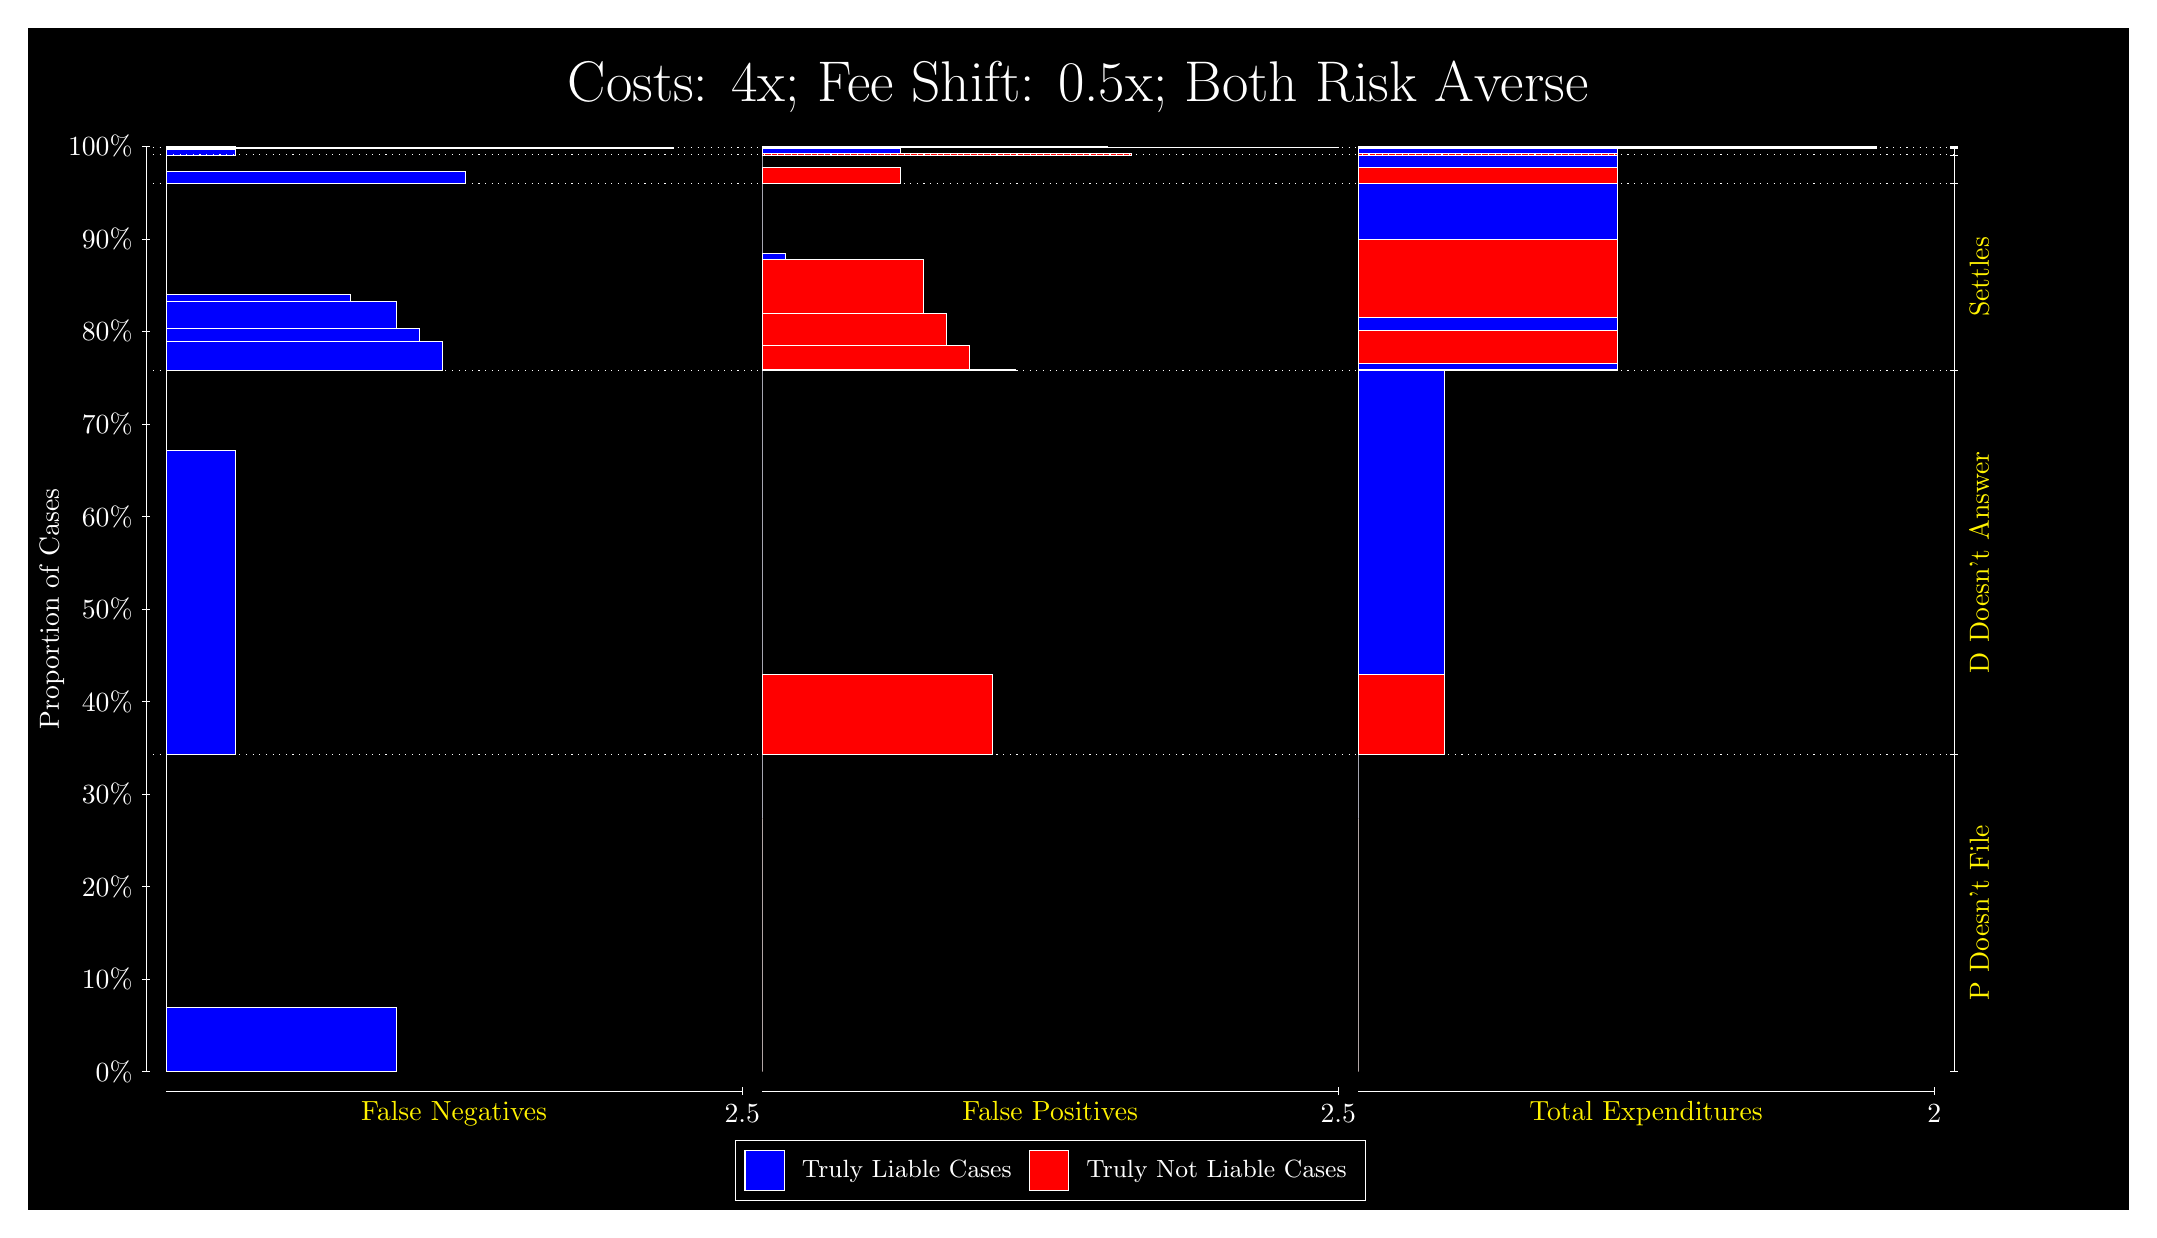
\begin{tikzpicture}
\draw[fill=black] (0,0) rectangle (26.667,15);
\draw[text=white] (0,13.5) rectangle (26.667,15) node[midway] {\huge Costs: 4x; Fee Shift: 0.5x; Both Risk Averse};
\draw[white, very thin] (1.5,1.75) -- (1.5,13.5);
\node[rotate=90, text=white, anchor=center] at (0.3, 7.625) {Proportion of Cases};
\draw[white, very thin] (1.45,1.75) -- (1.55,1.75);
\node[text=white, anchor=east] at (1.45, 1.75) {0\%};
\draw[white, very thin] (1.45,2.925) -- (1.55,2.925);
\node[text=white, anchor=east] at (1.45, 2.925) {10\%};
\draw[white, very thin] (1.45,4.1) -- (1.55,4.1);
\node[text=white, anchor=east] at (1.45, 4.1) {20\%};
\draw[white, very thin] (1.45,5.275) -- (1.55,5.275);
\node[text=white, anchor=east] at (1.45, 5.275) {30\%};
\draw[white, very thin] (1.45,6.45) -- (1.55,6.45);
\node[text=white, anchor=east] at (1.45, 6.45) {40\%};
\draw[white, very thin] (1.45,7.625) -- (1.55,7.625);
\node[text=white, anchor=east] at (1.45, 7.625) {50\%};
\draw[white, very thin] (1.45,8.8) -- (1.55,8.8);
\node[text=white, anchor=east] at (1.45, 8.8) {60\%};
\draw[white, very thin] (1.45,9.975) -- (1.55,9.975);
\node[text=white, anchor=east] at (1.45, 9.975) {70\%};
\draw[white, very thin] (1.45,11.15) -- (1.55,11.15);
\node[text=white, anchor=east] at (1.45, 11.15) {80\%};
\draw[white, very thin] (1.45,12.325) -- (1.55,12.325);
\node[text=white, anchor=east] at (1.45, 12.325) {90\%};
\draw[white, very thin] (1.45,13.5) -- (1.55,13.5);
\node[text=white, anchor=east] at (1.45, 13.5) {100\%};

\draw[white, very thin] (24.457,1.75) -- (24.457,13.5);
\draw[white, very thin] (24.407,1.75) -- (24.507,1.75);
\node[anchor=west] at (24.407, 1.75) {};
\draw[white, very thin] (24.407,5.7807) -- (24.507,5.7807);
\node[anchor=west] at (24.407, 5.7807) {};
\draw[white, very thin] (24.407,10.657) -- (24.507,10.657);
\node[anchor=west] at (24.407, 10.657) {};
\draw[white, very thin] (24.407,13.027) -- (24.507,13.027);
\node[anchor=west] at (24.407, 13.027) {};
\draw[white, very thin] (24.407,13.391) -- (24.507,13.391);
\node[anchor=west] at (24.407, 13.391) {};
\draw[white, very thin] (24.407,13.48) -- (24.507,13.48);
\node[anchor=west] at (24.407, 13.48) {};
\draw[white, very thin] (24.407,13.487) -- (24.507,13.487);
\node[anchor=west] at (24.407, 13.487) {};
\draw[white, very thin] (24.407,13.5) -- (24.507,13.5);
\node[anchor=west] at (24.407, 13.5) {};

\draw[white, very thin, fill=blue] (1.75,1.75) rectangle (4.6775,2.5662);
\draw[white, very thin, fill=red] (1.75,2.5662) rectangle (1.75,5.7807);
\draw[white, very thin, fill=blue] (1.75,5.7807) rectangle (2.6283,9.6386);
\draw[white, very thin, fill=red] (1.75,9.6386) rectangle (1.75,10.657);
\draw[white, very thin, fill=blue] (1.75,10.657) rectangle (5.2631,11.019);
\draw[white, very thin, fill=blue] (1.75,11.019) rectangle (4.9703,11.186);
\draw[white, very thin, fill=blue] (1.75,11.186) rectangle (4.6775,11.535);
\draw[white, very thin, fill=blue] (1.75,11.535) rectangle (4.3848,11.538);
\draw[white, very thin, fill=blue] (1.75,11.538) rectangle (4.092,11.618);
\draw[white, very thin, fill=red] (1.75,11.618) rectangle (1.75,13.027);
\draw[white, very thin, fill=blue] (1.75,13.027) rectangle (5.5558,13.186);
\draw[white, very thin, fill=red] (1.75,13.186) rectangle (1.75,13.391);
\draw[white, very thin, fill=blue] (1.75,13.391) rectangle (2.6283,13.459);
\draw[white, very thin, fill=red] (1.75,13.459) rectangle (1.75,13.48);
\draw[white, very thin, fill=blue] (1.75,13.48) rectangle (8.1906,13.483);
\draw[white, very thin, fill=red] (1.75,13.483) rectangle (1.75,13.487);
\draw[white, very thin, fill=blue] (1.75,13.487) rectangle (2.6283,13.497);
\draw[white, very thin, fill=red] (1.75,13.497) rectangle (1.75,13.5);
\draw[white, very thin, fill=red] (9.3189,1.75) rectangle (9.3189,4.9645);
\draw[white, very thin, fill=blue] (9.3189,4.9645) rectangle (9.3189,5.7807);
\draw[white, very thin, fill=red] (9.3189,5.7807) rectangle (12.246,6.7994);
\draw[white, very thin, fill=blue] (9.3189,6.7994) rectangle (9.3189,10.657);
\draw[white, very thin, fill=red] (9.3189,10.657) rectangle (12.539,10.667);
\draw[white, very thin, fill=red] (9.3189,10.667) rectangle (12.246,10.668);
\draw[white, very thin, fill=red] (9.3189,10.668) rectangle (11.954,10.971);
\draw[white, very thin, fill=red] (9.3189,10.971) rectangle (11.661,11.384);
\draw[white, very thin, fill=red] (9.3189,11.384) rectangle (11.368,12.067);
\draw[white, very thin, fill=blue] (9.3189,12.067) rectangle (9.6116,12.147);
\draw[white, very thin, fill=blue] (9.3189,12.147) rectangle (9.3189,13.027);
\draw[white, very thin, fill=red] (9.3189,13.027) rectangle (11.075,13.232);
\draw[white, very thin, fill=blue] (9.3189,13.232) rectangle (9.3189,13.391);
\draw[white, very thin, fill=red] (9.3189,13.391) rectangle (14.003,13.412);
\draw[white, very thin, fill=blue] (9.3189,13.412) rectangle (11.075,13.48);
\draw[white, very thin, fill=red] (9.3189,13.48) rectangle (11.075,13.484);
\draw[white, very thin, fill=blue] (9.3189,13.484) rectangle (9.3189,13.487);
\draw[white, very thin, fill=red] (9.3189,13.487) rectangle (16.638,13.49);
\draw[white, very thin, fill=blue] (9.3189,13.49) rectangle (13.71,13.5);
\draw[white, very thin, fill=red] (16.888,1.75) rectangle (16.888,4.9645);
\draw[white, very thin, fill=blue] (16.888,4.9645) rectangle (16.888,5.7807);
\draw[white, very thin, fill=red] (16.888,5.7807) rectangle (17.986,6.7994);
\draw[white, very thin, fill=blue] (16.888,6.7994) rectangle (17.986,10.657);
\draw[white, very thin, fill=red] (16.888,10.657) rectangle (20.181,10.667);
\draw[white, very thin, fill=blue] (16.888,10.667) rectangle (20.181,10.747);
\draw[white, very thin, fill=red] (16.888,10.747) rectangle (20.181,11.159);
\draw[white, very thin, fill=blue] (16.888,11.159) rectangle (20.181,11.327);
\draw[white, very thin, fill=red] (16.888,11.327) rectangle (20.181,12.314);
\draw[white, very thin, fill=blue] (16.888,12.314) rectangle (20.181,13.027);
\draw[white, very thin, fill=red] (16.888,13.027) rectangle (20.181,13.232);
\draw[white, very thin, fill=blue] (16.888,13.232) rectangle (20.181,13.391);
\draw[white, very thin, fill=red] (16.888,13.391) rectangle (20.181,13.412);
\draw[white, very thin, fill=blue] (16.888,13.412) rectangle (20.181,13.48);
\draw[white, very thin, fill=red] (16.888,13.48) rectangle (23.475,13.484);
\draw[white, very thin, fill=blue] (16.888,13.484) rectangle (23.475,13.487);
\draw[white, very thin, fill=red] (16.888,13.487) rectangle (23.475,13.49);
\draw[white, very thin, fill=blue] (16.888,13.49) rectangle (23.475,13.5);
\draw[white, dotted] (1.5,5.7807) -- (24.457,5.7807);
\draw[white, dotted] (1.5,10.657) -- (24.457,10.657);
\draw[white, dotted] (1.5,13.027) -- (24.457,13.027);
\draw[white, dotted] (1.5,13.391) -- (24.457,13.391);
\draw[white, dotted] (1.5,13.48) -- (24.457,13.48);
\draw[white, dotted] (1.5,13.487) -- (24.457,13.487);
\draw[white, very thin] (1.75,1.5) -- (9.0689,1.5);
\node[text=yellow, anchor=north] at (5.4094, 1.5) {False Negatives};
\draw[white, very thin] (9.0689,1.45) -- (9.0689,1.55);
\node[text=white, anchor=north] at (9.0689, 1.45) {2.5};

\draw[white, very thin] (9.3189,1.5) -- (16.638,1.5);
\node[text=yellow, anchor=north] at (12.978, 1.5) {False Positives};
\draw[white, very thin] (16.638,1.45) -- (16.638,1.55);
\node[text=white, anchor=north] at (16.638, 1.45) {2.5};

\draw[white, very thin] (16.888,1.5) -- (24.207,1.5);
\node[text=yellow, anchor=north] at (20.547, 1.5) {Total Expenditures};
\draw[white, very thin] (24.207,1.45) -- (24.207,1.55);
\node[text=white, anchor=north] at (24.207, 1.45) {2};

\node[text=yellow, centered, rotate=90] at (24.777, 3.7653) {P Doesn't File};
\node[text=yellow, centered, rotate=90] at (24.777, 8.219) {D Doesn't Answer};
\node[text=yellow, centered, rotate=90] at (24.777, 11.842) {Settles};





\draw (12.978300999999998,1.5) node[draw=none] (baseCoordinate) {};
\begin{scope}[align=center]
        \matrix[scale=0.5, draw=white, below=0.5cm of baseCoordinate, nodes={draw}, column sep=0.1cm]{
            \node[rectangle, draw, minimum width=0.5cm, minimum height=0.5cm, fill=blue] {}; &
            \node[draw=none, font=\small, text=white] (B) {Truly Liable Cases}; &
            \node[rectangle, draw, minimum width=0.5cm, minimum height=0.5cm, fill=red] {}; &
            \node[draw=none, font=\small, text=white] (B) {Truly Not Liable Cases}; \\
            };
\end{scope}

\end{tikzpicture}
\end{document}